% Created 2014-08-20 Wed 16:11
\documentclass[table,smaller]{beamer}
\usepackage[utf8]{inputenc}
\usepackage[T1]{fontenc}
\usepackage{fixltx2e}
\usepackage{graphicx}
\usepackage{longtable}
\usepackage{float}
\usepackage{wrapfig}
\usepackage{rotating}
\usepackage[normalem]{ulem}
\usepackage{amsmath}
\usepackage{textcomp}
\usepackage{marvosym}
\usepackage{wasysym}
\usepackage{amssymb}
\usepackage{hyperref}
\tolerance=1000
\usepackage{tikz}
\usepackage{minted}
\usepackage{fancyvrb}
\usemintedstyle{perldoc}
\definecolor{lightgray}{gray}{0.96}
\setlength{\tabcolsep}{1ex}
\institute{Harvard MIT Data Center}
\usetheme{Warsaw}
\useoutertheme{infolines}
\setbeamercolor{block body}{bg=lightgray}
\titlegraphic{
\includegraphics[width=.75\textwidth]{images/IQSSNewLogo.pdf}}
\setbeamersize{text margin left=2em,text margin right=2em}
\AtBeginSection[]{\begin{frame}<beamer>\frametitle{Topic}\tableofcontents[currentsection]\end{frame}}
\usetheme{default}
\author{Ista Zahn}
\date{}
\title{Introduction to Stata}
\hypersetup{
  pdfkeywords={},
  pdfsubject={},
  pdfcreator={Emacs 24.3.1 (Org mode 8.2.7c)}}
\begin{document}

\maketitle
\begin{frame}{Outline}
\tableofcontents
\end{frame}



\section{Introduction}
\label{sec-1}

\begin{frame}[label=sec-1-1]{Documents for today}
USERNAME: dataclass
PASSWORD: dataclass
\begin{itemize}
\item Find class materials at \url{http://j.mp/intro-stata}
\item Download and extract to your desktop!
\end{itemize}
\end{frame}

\begin{frame}[label=sec-1-2]{Organization}
\begin{itemize}
\item Please feel free to ask questions at any point if they are relevant to the current topic (or if you are lost!)
\begin{itemize}
\item There will be a Q\&A after class for more specific, personalized questions
\end{itemize}
\item Collaboration with your neighbors is encouraged
\item If you are using a laptop, you will need to adjust paths accordingly
\item Make comments in your Do-file rather than on hand-outs  
\begin{itemize}
\item save on flash drive or email to yourself
\end{itemize}
\end{itemize}
\end{frame}

\begin{frame}[label=sec-1-3]{Workshop descripton}
\begin{itemize}
\item This is an \alert{introduction} to Stata
\item Assumes no/very little knowledge of Stata
\item Not appropriate for people already well familiar with Stata
\item Learning Objectives:
\begin{itemize}
\item Familiarize yourself with the Stata interface
\item Get data in and out of Stata
\item Compute statistics and construct graphical displays
\item Compute new variables and transformations
\end{itemize}
\end{itemize}
\end{frame}

\begin{frame}[label=sec-1-4]{Why stata?}
\begin{itemize}
\item Used in a variety of disciplines
\item User-friendly
\item Great guides available on web (as well as in HMDC computer lab library)
\item Student and other discount packages available at reasonable cost
\end{itemize}
\end{frame}

\begin{frame}[label=sec-1-5]{Stata interface}
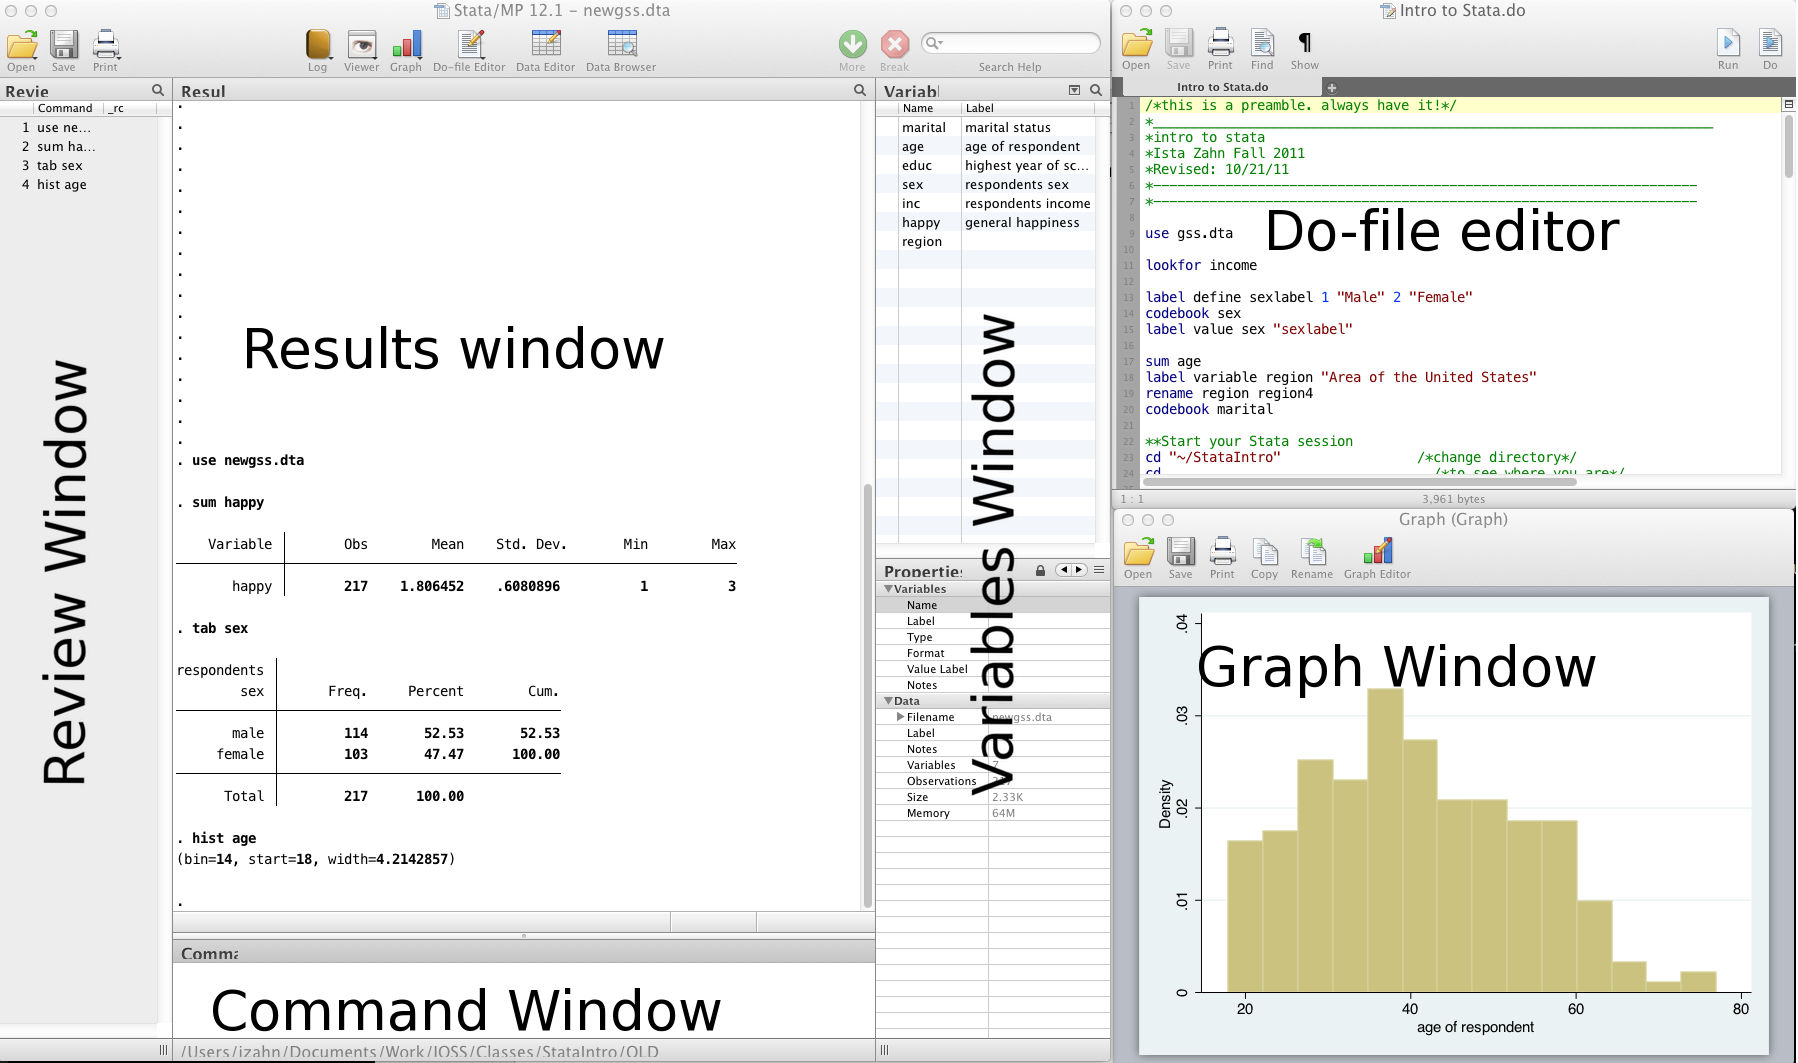
\includegraphics[width=.9\linewidth]{images/StataInterface.png}

\begin{itemize}
\item Review and Variable windows can be closed (user preference)
\item Command window can be shortened (recommended)
\end{itemize}
\end{frame}

\begin{frame}[label=sec-1-6]{Do-files}
\begin{itemize}
\item You can type all the same commands into the Do-file that you would type into the command window
\item BUT\ldots{}the Do-file allows you to \alert{save} your commands
\item Your Do-file should contain ALL commands you executed -- at least all the "correct" commands!
\item I recommend never using the command window or menus to make CHANGES to data
\item Saving commands in Do-file allows you to keep a written record of everything you have done to your data
\begin{itemize}
\item Allows easy replication
\item Allows you to go back and re-run commands,  analyses and make modifications
\end{itemize}
\end{itemize}
\end{frame}


\begin{frame}[label=sec-1-7]{Stata help}
\begin{itemize}
\item Easiest way to get help in Stata - just type \alert{help} followed by topic or command, e.g., 
\alert{help regress}
\item Falls back to "search" if command not found
\item Generally, if you google "Stata [topic]," you'll get some helpful hits
\item UCLA website:
\url{http://www.ats.ucla.edu/stat/Stata/}
\end{itemize}
\end{frame}

\begin{frame}[label=sec-1-8]{General Stata command syntax}
\begin{itemize}
\item Most Stata commands follow the same underlying principles
\alert{Command varlist, options}, e.g., \alert{sum var1 var2, detail}
\begin{itemize}
\item CAUTION - in some cases, if you type a command and don't specify a variable, Stata will perform the command on all variables in your dataset
\end{itemize}
\item You can find command-specific syntax in the help files
\end{itemize}
\end{frame}

\begin{frame}[fragile,label=sec-1-9]{Commenting and formatting syntax}
 \begin{itemize}
\item Start with comment describing your Do-file and use comments throughout
\item Single line and block comments
\end{itemize}
\vspace{-.5em} \begin{columns} \column{.85\linewidth} \begin{block}{}
\begin{minted}[fontsize=\footnotesize]{c}
// comment
 describe var
 /*
 comment block comment block comment block comment
 block comment block comment block 
*/
\end{minted}
\end{block} \end{columns}

\begin{itemize}
\item Use \emph{/} to break varlists over multiple lines:
\end{itemize}
\vspace{-.5em} \begin{columns} \column{.85\linewidth} \begin{block}{}
\begin{minted}[fontsize=\footnotesize]{c}
// break commands over multible lines
describe var1 var2 var2 ///
var4 var5 var6
\end{minted}
\end{block} \end{columns}
\end{frame}


\begin{frame}[fragile,label=sec-1-10]{Let's get started}
 \begin{itemize}
\item Launch the Stata program (MP or SE, does not matter unless doing computationally intensive work)
\begin{itemize}
\item Open up a new Do-file
\item Run our first Stata code!
\end{itemize}
\end{itemize}

\vspace{-.5em} \begin{columns} \column{.85\linewidth} \begin{block}{}
\begin{minted}[fontsize=\footnotesize]{c}
// change directory
cd "C://Users/dataclass/Desktop/StataIntro"
// start a log file to record your stata session
log using myStataLog.txt, text replace
// Pause / resume logging with "log on" / "log off"
// Close lot with "log close"
\end{minted}
\end{block} \end{columns}
\end{frame}

\begin{frame}[label=sec-1-11]{How to start every do-file}
\begin{enumerate}
\item Describe what the file does
\item Change directory
\item Begin log file
\item Call up data
\item Do stuff: Data manipulation, statistics etc.
\item Save data under new name (if making changes to dataset)
\end{enumerate}
\end{frame}



\section{Getting data into Stata}
\label{sec-2}


\begin{frame}[fragile,label=sec-2-1]{Data file commands}
 \begin{itemize}
\item Next, we want to open our data file
\item Open/save data sets with "use" and "save":
\end{itemize}

\vspace{-.5em} \begin{columns} \column{.85\linewidth} \begin{block}{}
\begin{minted}[fontsize=\footnotesize]{c}
cd dataSets
// open the gss.dta data set
use gss.dta
// saving your data file:
save newgss.dta, replace
// the "replace" option tells stata it's OK to 
//   write over an existing file
\end{minted}

\end{block} \end{columns}
\end{frame}

\begin{frame}[label=sec-2-2]{A note about path names}
\begin{itemize}
\item If your path has no spaces in the name (that means all directories, folders, file names, etc. can have no spaces), you can write the path as is
\item If there are spaces, you need to put your pathname in quotes
\item Best to get in the habit of quoting paths
\end{itemize}
\end{frame}

\begin{frame}[label=sec-2-3]{Where's my data?}
\begin{itemize}
\item Data editor (\alert{browse})
\item Data editor (\alert{edit})
\begin{itemize}
\item Using the data editor is discouraged (why?)
\end{itemize}
\item Always keep any changes to your data in your Do-file
\item Avoid temptation of making manual changes by viewing data via the browser rather than editor
\end{itemize}
\end{frame}

\begin{frame}[fragile,label=sec-2-4]{What if my data is not a Stata file?}
 \begin{itemize}
\item Import delimited text files
\end{itemize}
\vspace{-.5em} \begin{columns} \column{.85\linewidth} \begin{block}{}
\begin{minted}[fontsize=\footnotesize]{c}
/* import data from a .csv file */
insheet using gss.csv, clear
/* save data to a .csv file */
outsheet using gss_new.csv, replace comma
\end{minted}

\end{block} \end{columns}

\begin{itemize}
\item Import data from SAS and Excel
\end{itemize}
\vspace{-.5em} \begin{columns} \column{.85\linewidth} \begin{block}{}
\begin{minted}[fontsize=\footnotesize]{c}
/* import/export SAS xport files */
clear
import sasxport gss.xpt
export sasxport newFileName, replace

/* import/export data from Excel */
import excel using gss.xlsx, firstrow clear
export excel newFileName.xls, replace
\end{minted}

\end{block} \end{columns}
\end{frame}

\begin{frame}[label=sec-2-5]{What if my data is from another statistical software program?}
\begin{itemize}
\item SPSS/PASW will allow you to save your data as a Stata file
\begin{itemize}
\item Go to: file > save as > Stata (use most   recent version available)
\item Then you can just go into Stata and   open it
\end{itemize}
\item Another option is \alert{StatTransfer}, a program that converts data from/to many common formats, including SAS, SPSS, Stata, and many more
\end{itemize}
\end{frame}

\begin{frame}[label=sec-2-6]{Exercise 1: Importing data}
\begin{enumerate}
\item Close down Stata and open a new session
\item Go through the three steps for starting each Stata  session that we reviewed
\begin{itemize}
\item Begin a log file
\item Open your Stata dataset (gss.dta)
\item Save your Stata dataset using a different name
\end{itemize}
\item Try opening the following files:
\begin{itemize}
\item A comma separated value file: gss.csv
\item A SPSS file: gss.sav
\item A SAS transport file: gss.xpt
\end{itemize}
\end{enumerate}
\end{frame}


\section{Statistics and graphs}
\label{sec-3}

\begin{frame}[fragile,label=sec-3-1]{Basic graphing commands}
 \begin{itemize}
\item Univariate distribution(s) using \alert{hist}
\end{itemize}
\vspace{-.5em} \begin{columns} \column{.85\linewidth} \begin{block}{}
\begin{minted}[fontsize=\footnotesize]{c}
/* Histograms */
hist educ
// histogram with normal curve; see 'help hist' for other options
hist age, normal
\end{minted}

\end{block} \end{columns}

\begin{itemize}
\item View bivariate distributions with scatterplots
\end{itemize}
\vspace{-.5em} \begin{columns} \column{.85\linewidth} \begin{block}{}
\begin{minted}[fontsize=\footnotesize]{c}
/* scatterplots */
twoway (scatter educ age)
graph matrix educ age inc
\end{minted}

\end{block} \end{columns}
\end{frame}

\begin{frame}[fragile,label=sec-3-2]{The "by" command}
 \begin{itemize}
\item Sometimes, you'd like to generate  output based on different categories of a grouping variable
\item The "by" command does just this
\end{itemize}

\vspace{-.5em} \begin{columns} \column{.85\linewidth} \begin{block}{}
\begin{minted}[fontsize=\footnotesize]{c}
/* By Processing */
// tabulate happy separately for men and women
bysort sex: tab happy
// summarize eudcation by marital status
bysort marital: sum educ
\end{minted}

\end{block} \end{columns}
\end{frame}


\begin{frame}[label=sec-3-3]{Exercise 2: Descriptive statistics}
\begin{enumerate}
\item Use the dataset, gss.dta
\item Examine a few selected variables using the describe, sum and codebook commands
\item Tabulate the variable, "marital," with and without labels
\item Summarize the variable, "income" separately participants based on marital status
\item Cross-tabulate marital with region and show gender percent by region
\item Summarize the variable, "happy" for married individuals only
\item Generate a histogram of income
\item Generate a second histogram of income, but this time, split income based on participants sex and ask Stata to print the normal curve on your histograms
\end{enumerate}
\end{frame}


\section{Basic data management}
\label{sec-4}

\begin{frame}[label=sec-4-1]{Labels}
\begin{itemize}
\item You never know why and when your data may be reviewed
\item ALWAYS label every variable no matter how insignificant it may seem
\item Stata uses two sets of labels: \alert{variable labels} and \alert{value labels}
\item Variable labels are very easy to use -- value labels are a little more complicated
\end{itemize}
\end{frame}

\begin{frame}[fragile,label=sec-4-2]{Variable and value labels}
 \begin{itemize}
\item Variable labels
\end{itemize}
\vspace{-.5em} \begin{columns} \column{.85\linewidth} \begin{block}{}
\begin{minted}[fontsize=\footnotesize]{c}
/* Labelling and renaming */
// Label variable inc "household income"
label var inc "household income"

// change the name 'educ' to 'education'
rename educ education

// you can search names and labels with 'lookfor' 
lookfor household
\end{minted}

\end{block} \end{columns}

\begin{itemize}
\item Value labels are a two step process: define a value label, then assign defined label to variable(s)
\end{itemize}

\vspace{-.5em} \begin{columns} \column{.85\linewidth} \begin{block}{}
\begin{minted}[fontsize=\footnotesize]{c}
/*define a value label for sex */
label define mySexLabel 1 "Male" 2 "Female"
/* assign our label set to the sex variable*/
label val sex  mySexLabel
\end{minted}

\end{block} \end{columns}
\end{frame}

\begin{frame}[label=sec-4-3]{Exercise 3: Variable labels and value labels}
\begin{enumerate}
\item Open the data set \alert{gss.csv}
\item Familiarize yourself with the  data using describe, sum, etc.
\item Rename and label variables using the following codebook:
\end{enumerate}
{ \scriptsize
\begin{center}
\begin{tabular}{lll}
\alert{var} & \alert{rename to} & \alert{label with}\\
\hline
v1 & marital & marital status\\
v2 & age & age of respondent\\
v3 & educ & education\\
v4 & sex & respondent's sex\\
v5 & inc & household income\\
v6 & happy & general happiness\\
v7 & region & region of interview\\
\hline
\end{tabular}
\end{center}
}
\begin{enumerate}
\item Add value labels to your "marital" variable using this codebook:
\end{enumerate}
{ \scriptsize
\begin{center}
\begin{tabular}{rl}
\alert{value} & \alert{label}\\
\hline
1 & "married"\\
2 & "widowed"\\
3 & "divorced"\\
4 & "separated"\\
5 & "never married"\\
\hline
\end{tabular}
\end{center}
}
\end{frame}

\begin{frame}[label=sec-4-4]{Working on subsets}
\begin{itemize}
\item It is often useful to select just those rows of your data where some condition holds--for example select only rows where sex is 1 (male)
\item The following operators allow you to do this:
\begin{description}
\item[{==}] equal to
\item[{!=}] not equal to
\item[{>}] greater than
\item[{<}] less than
\item[{>=}] greater than or equal to
\item[{<=}] less than or equal to
\item[{\&}] and
\item[{|}] or
\end{description}
\item Note the double equals signs for testing equality
\end{itemize}
\end{frame}

\begin{frame}[fragile,label=sec-4-5]{Generating and replacing variables}
 \begin{itemize}
\item Create new variables using "gen"
\end{itemize}
\vspace{-.5em} \begin{columns} \column{.85\linewidth} \begin{block}{}
\begin{minted}[fontsize=\footnotesize]{c}
// create a new variable named mc_inc
//   equal to inc minus the mean of inc
gen mc_inc = inc - 15.37
\end{minted}

\end{block} \end{columns}

\begin{itemize}
\item Sometimes useful to start with blank values and fill them in based on values of existing variables
\end{itemize}

\vspace{-.5em} \begin{columns} \column{.85\linewidth} \begin{block}{}
\begin{minted}[fontsize=\footnotesize]{c}
/* the 'generate and replace' strategy */ 
// generate a column of missings
gen age_wealth = .
// Next, start adding your qualifications
replace age_wealth=1 if age<30 & inc < 10
replace age_wealth=2 if age<30 & inc > 10
replace age_wealth=3 if age>30 & inc < 10
replace age_wealth=4 if age>30 & inc > 10

// conditions can also be combined with "or"
gen young=0
replace young=1 if age_wealth==1 | age_wealth==2
\end{minted}

\end{block} \end{columns}
\end{frame}

\begin{frame}[label=sec-4-6]{Exercise 4: Manipulating variables}
\begin{enumerate}
\item Use the dataset, gss.dta
\item Generate a new variable, age2 equal to age squared
\item Generate a new "high income" variable that will take on a value of "1" if a person has an income value greater than "15" and "0" otherwise
\item Generate a new divorced/separated dummy variable that will take on a value of "1" if a person is either divorced or separated and "0" otherwise
\end{enumerate}
\end{frame}


\section{Wrap-up}
\label{sec-5}

\begin{frame}[label=sec-5-1]{Help us make this workshop better!}
\begin{itemize}
\item Please take a moment to fill out a very short feedback form

\item These workshops exist for you – tell us what you need!

\item \url{http://tinyurl.com/6h3cxnz}
\end{itemize}
\end{frame}


\begin{frame}[label=sec-5-2]{Additional resources}
\begin{itemize}
\item IQSS workshops: \url{http://projects.iq.harvard.edu/rtc/filter_by/workshops}

\item IQSS statistical consulting: \url{http://rtc.iq.harvard.edu}

\item The RCE
\begin{itemize}
\item Research Computing Enviroment (RCE) service available to Harvard \& MIT users
\item \texttt{www.iq.harvard.edu/research\_computing}
\item Wonderful resource for organizing data, running analyses efficiently
\item Creates a centralized place to store data and run analysis
\item Supplies persistent desktop environment accessible from any computer with an internet connection
\end{itemize}
\end{itemize}
\end{frame}
% Emacs 24.3.1 (Org mode 8.2.7c)
\end{document}